\section{Named Data Networking (NDN)}
\label{sec:ndn}

In the Named Data Networking (NDN)~\cite{Jacobson2009} architecture, 
clients issue subscriptions for content 
objects by specifying 
a hierarchical (URL-like) content name, e.g. 
\verb+/pdeec+\addthinspace\verb+/mtsp/+\addthinspace\verb+2014/+, which is 
directly used in NDN packets. 
Destination network locators (e.g. IP addresses) are not used in this case, as 
NDN routers are able 
to forward such packets towards appropriate content-holding destinations, solely based 
on such names. NDN contemplates two fundamental types of packets, `Interest' and `Data' packets, 
used for content subscriptions and publications, respectively. Interest packets 
are originally released into the network by clients willing to access a 
particular content, addressing it via its content name, while Data packets 
carry the content itself.\shortvertbreak

\begin{figure}[h!]

    \centering
    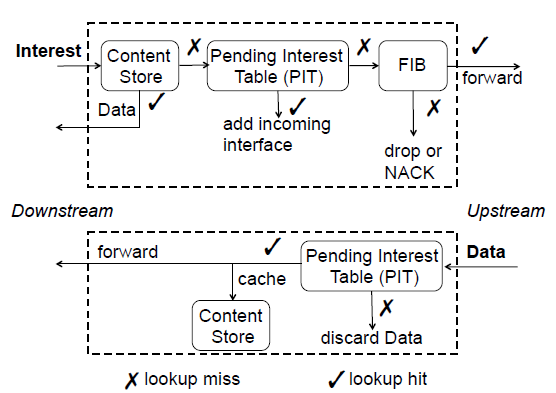
\includegraphics[width=0.35\textwidth]{figures/ndn-forwarding-engine.png}
    \cprotect\caption{Interest and Data packet processing according to NDN's 
        forwarding engine~\cite{Yi2012}.}
    \label{fig:ccn-icn-ndn-forwarding-engine}

\end{figure}

An NDN router is conceptually composed by three main elements: (1) a 
Forward Information 
Base (FIB), (2) a Pending Interest Table (PIT) and (3) a Content Store 
(CS)~\cite{Jacobson2009}:

\begin{itemize}

    \item \textbf{Forward Information Base (FIB):} Routing\slash forwarding 
        table holding entries 
        which relate a name prefix and a list of router interfaces to which 
        Interest packets matching that content name prefix should be forwarded 
        to.
    \item \textbf{Pending Interest Table (PIT):} A table which keeps track of 
        the mapping between arriving Interest packets and 
        the interfaces these have been received from, in order to save a reverse 
        path for Data packets 
        towards one or more subscribers (this may be a 1:N mapping, as an 
        Interest packet matching the same content may be received in 
        multiple interfaces).
    \item \textbf{Content Store (CS):} A cache for content, indexed by content 
        name or item. This novel element allows for content storage at the 
        network level. In-network caching allows an Interest to be satisfied 
        by a matching Data packet in any location other than the original 
        producer of the content, constituting one of the main 
        content-oriented characteristics of NDN.

\end{itemize}

In NDN, communication is receiver-driven, i.e. having the desire to fetch 
a particular content, a client releases an Interest packet into the network 
so that it is forwarded towards an appropriate content holder. In 
Figure~\ref{fig:ccn-icn-ndn-forwarding-engine}~\cite{Yi2012}, we provide a 
graphical description 
of the mechanics of the forwarding engine of an NDN router, supported by 
the textual description provided below:

\begin{enumerate}

    \item An Interest packet arrives on an interface (e.g. \verb+iface0+) of an NDN router.
    \item A longest prefix match on the content name specified in the Interest (e.g. \verb+name+) 
        is performed. The NDN router will now look in its CS, PIT and FIB, in 
        that order, in order to resume the forwarding action:
        \begin{enumerate}

            \item If there's a match in the router's CS, a copy of the respective 
                CS entry will be sent back via \verb+iface0+, the Interest 
                packet is dropped. Depending on the pre-specified 
                caching policy (e.g. MRU, LRU, LFU~\footnote{\url{http://en.wikipedia.org/wiki/Cache_algorithms}}, 
                etc.), the organization of the CS 
                may change at this point. \textbf{End.}

            \item Else if there is an (exact) match in the PIT, \verb+iface0+ is 
                added to the mapping list on the respective entry. The 
                Interest packet is dropped (as a previous one has already been 
                sent upstream). \textbf{End.}

            \item Else if only a matching FIB entry is found, the Interest 
                packet is forwarded upstream, via all remaining interfaces on the 
                list (except \verb+iface0+), towards an eventual content holder. A PIT 
                entry $<$\verb+name+, \verb+iface0+$>$ is added. \textbf{End.}

            \item Else if there is no match at all, the Interest packet is 
                simply discarded. \textbf{End.}\shortvertbreak

        \end{enumerate}

\end{enumerate}

Note that in NDN only Interest packets are forwarded: intermediate NDN 
routers (i.e. between client and content holder) forward the 
Interests and have their respective PIT tables updated with Interest-to-interface 
mappings, pre-establishing a reverse path for Data packets to follow as soon as a 
content holder is found. When the reverse path is `followed' (i.e. in the 
`downstream' direction, lower part of Figure~\ref{fig:ccn-icn-ndn-forwarding-engine}), each 
intermediate NDN router receiving a 
Data packet looks in its PIT for $<$\verb+name+, \verb+iface+$>$ entries, 
and forwards the Data packet through all matching interfaces. In addition, a 
CS entry is created to cache the content locally at the router (again, depending 
on the caching policy, the organization of the CS may change at this point). If a Data packet 
with no matching PIT entries arrives, it is treated as unsolicited and discarded.

